\documentclass[]{article}

% Imported Packages
%------------------------------------------------------------------------------
\usepackage{amssymb}
\usepackage{amstext}
\usepackage{amsthm}
\usepackage{amsmath}
\usepackage{enumerate}
\usepackage{fancyhdr}
\usepackage[margin=1in]{geometry}
\usepackage{graphicx}
\usepackage{extarrows}
\usepackage{setspace}
%------------------------------------------------------------------------------

% Header and Footer
%------------------------------------------------------------------------------
\pagestyle{plain}  
\renewcommand\headrulewidth{0.4pt}                                      
\renewcommand\footrulewidth{0.4pt}                                    
%------------------------------------------------------------------------------

% Title Details
%------------------------------------------------------------------------------
\title{Deliverable \#3}
\author{SE 3A04: Software Design II -- Large System Design}
\date{}     
%------------------------------------------------------------------------------

% Document
%------------------------------------------------------------------------------
\begin{document}

\maketitle	

{\noindent\bf Group Number:} G8 \\
{\bf Group Members:} 
\begin{itemize}
	\item Hashim Bukhtiar
	\item Jaden Moore
	\item James Ariache
	\item Olivia Reich
	\item Omar Abdelhamid
\end{itemize}

\section{Introduction}
\label{sec:introduction}
% Begin Section

\subsection{Purpose}
\label{sub:purpose}
% Begin SubSection

This document provides further information about the RideRecon car identification system architecture, including state chart diagrams, sequence diagrams, and a detailed class diagram. This document is intended for internal RideRecon stakeholders, including but not limited to, project managers, developers, domain experts, and RideRecon team members/investors. \\

\noindent RideRecon Deliverable 1 and 2 should be read prior, and technical knowledge may be beneficial in better understanding the contents of the document.


% End SubSection

\subsection{System Description}
\label{sub:system_description}
% Begin SubSection

The RideRecon system is a vehicle identification platform that processes user-provided text and image inputs to accurately recognize and classify cars. The system leverages a hybrid blackboard-repository architecture, where multiple expert modules—including a trained ML model (G8M), a reverse image search engine, vector imaging techniques, and GPT-based text processing—collaborate to determine the most accurate identification. The blackboard component acts as a shared workspace where expert modules contribute insights, iteratively refining the identification, while the repository component ensures efficient data management, storing user inputs, past identifications, and expert processing outcomes for future reference.\\

\noindent This document builds on the foundational system description provided in Deliverable 2, expanding the technical details through state charts, sequence diagrams, and a detailed class diagram. These artifacts provide a deeper understanding of the system’s data flow, processing logic, and user interactions. The diagrams illustrate how user inputs progress through various system components, from input validation to expert analysis and final result generation. Additionally, this document clarifies how user accounts, history tracking, and car collection management integrate into the broader system. Through these detailed design elements, we establish a clear roadmap for the system’s implementation and behavior.

% End SubSection

\subsection{Overview}
\label{sub:overview}
% Begin SubSection
This document provides a structured analysis and design of the \textbf{RideRecon} system, focusing on the \textbf{State Chart Diagrams}, \textbf{Sequence Diagrams}, and a detailed \textbf{Class Diagram}. It expands upon the foundational concepts introduced in \textbf{Deliverables 1 and 2}, ensuring a comprehensive understanding of the system's behavior and interactions.\\
 
\noindent\textbf{Section 2} presents \textbf{State Chart Diagrams}, which define the behavior of core controller classes, particularly focusing on user management and vehicle identification. These diagrams illustrate the different states a system entity can transition between and the conditions that trigger these transitions. \textbf{Section 3} provides \textbf{Sequence Diagrams}, visually representing the flow of interactions between system components during specific use cases. These diagrams capture step-by-step interactions between users, expert modules, and the system’s processing units. \textbf{Section 4} contains the \textbf{Class Diagram}, outlining the structure of the system’s classes, their attributes, relationships, and methods. This diagram ensures clarity in class responsibilities, making it easier to understand how data is managed within the system.\\
 
\noindent Together, these sections form a comprehensive guide to understanding the \textbf{RideRecon system’s state management, process flow, and class relationships}, providing essential details for implementation and further development.

 

% End SubSection

% End Section

\section{State Charts for Controller Classes}
\label{sec:state_charts_for_controller_classes}
% Begin Section

\begin{center}
	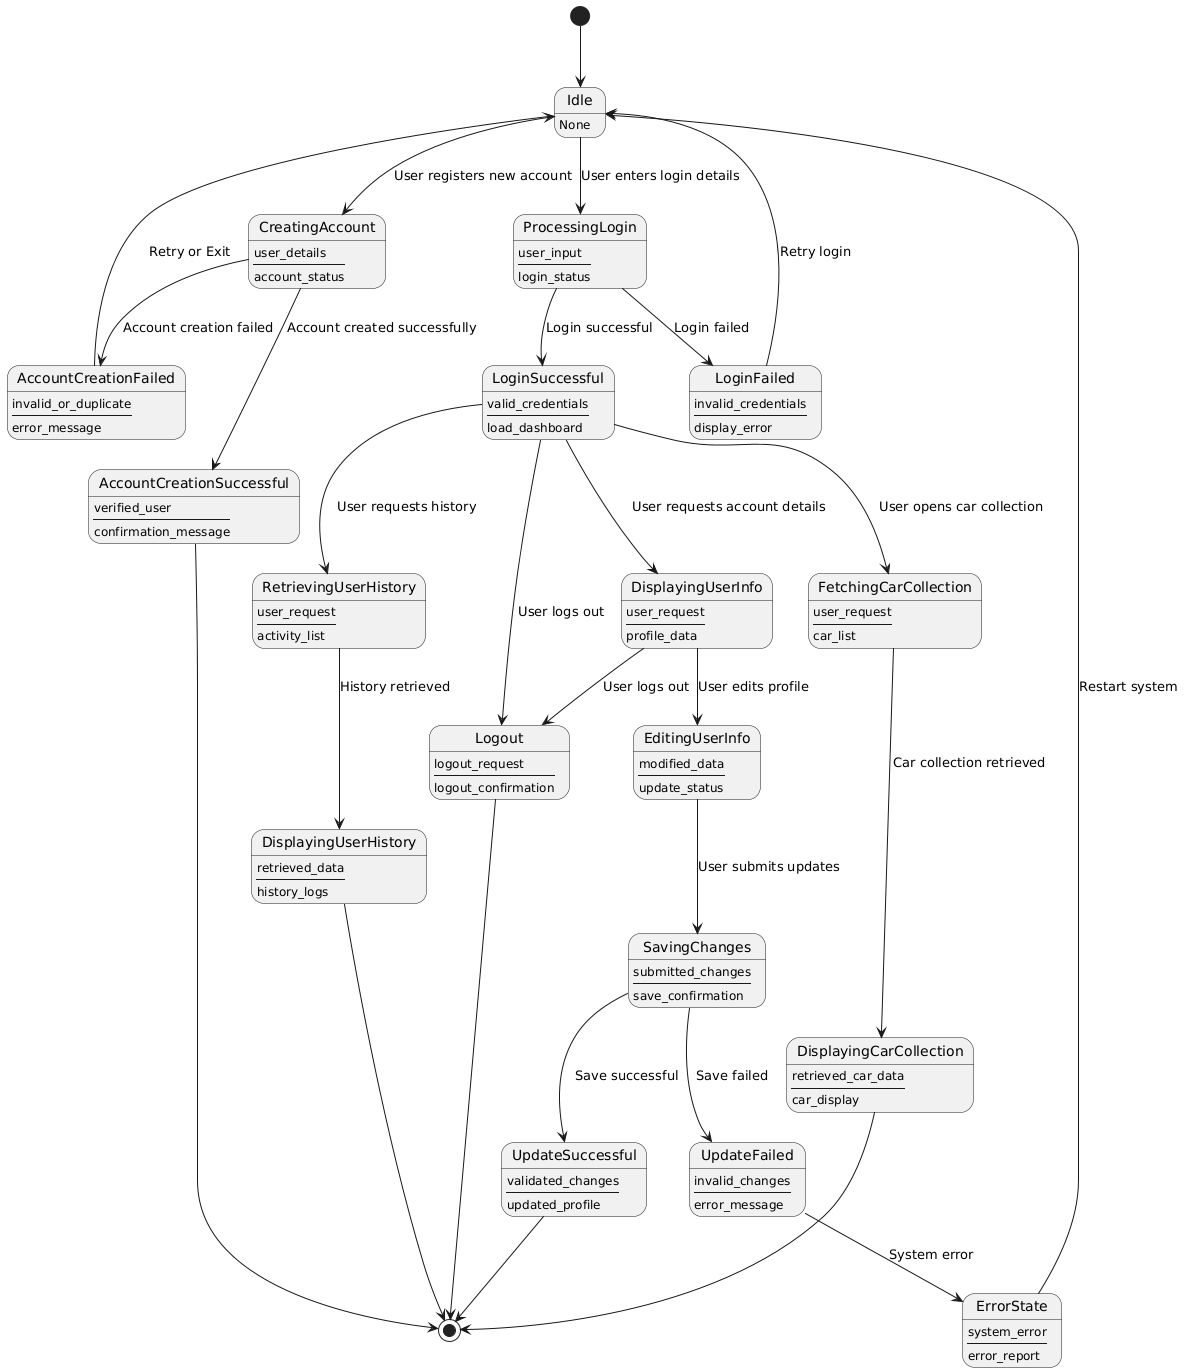
\includegraphics[scale=0.43]{State Diagrams/omar_diagram.png}\\
	\textbf{Figure 1.} State Chart Diagram for User Manager.\\

	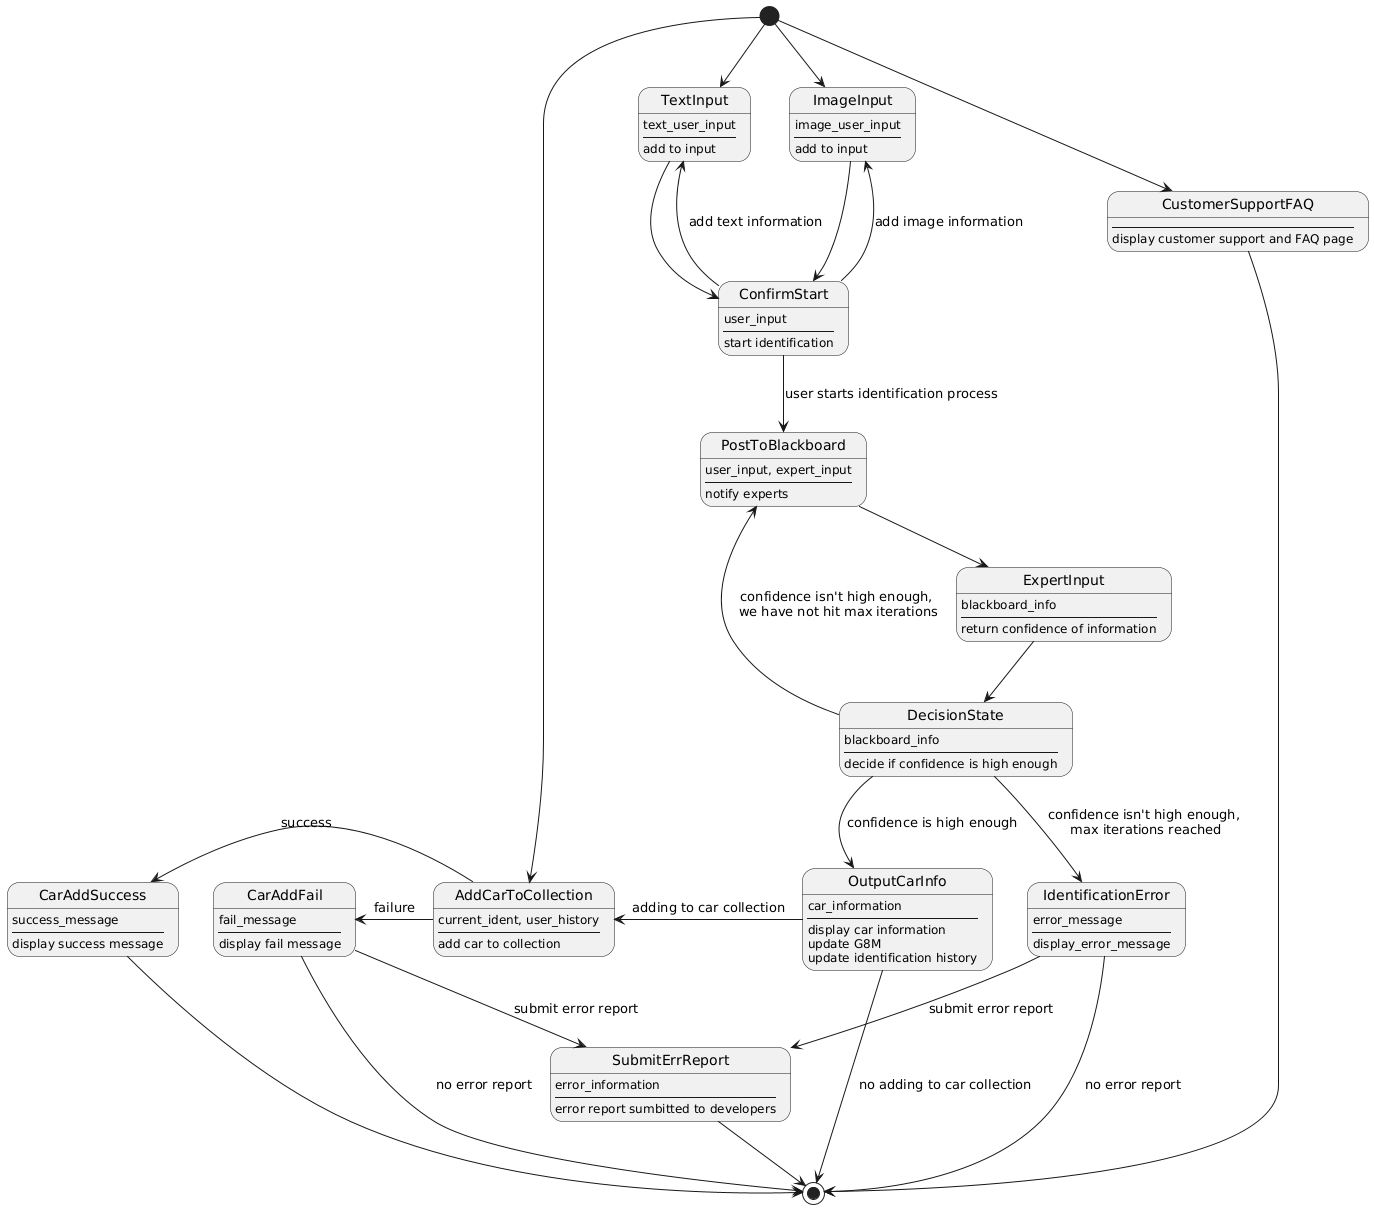
\includegraphics[scale=0.38]{State Diagrams/IdentStateDiagramUML.png}\\ 
	\textbf{Figure 2.} State Chart Diagram for Identification Manager.\\
\end{center}

% End Section

\section{Sequence Diagrams}
\label{sec:sequence_diagrams}
% Begin Section


\begin{center}
	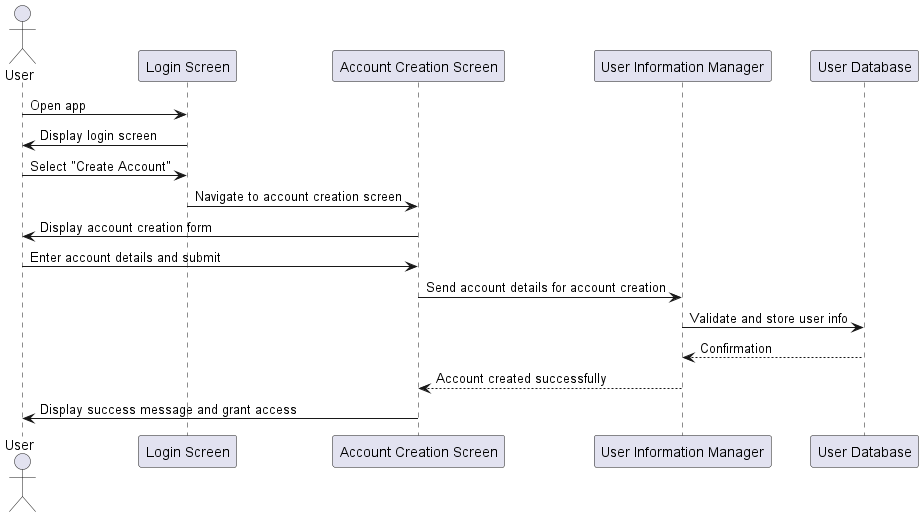
\includegraphics[scale=0.5]{Sequence Diagrams/BE1_Sequence_Diagram.png}\\
	\textbf{Figure 3.} Sequence Diagram for BE1: Create Account.\\

	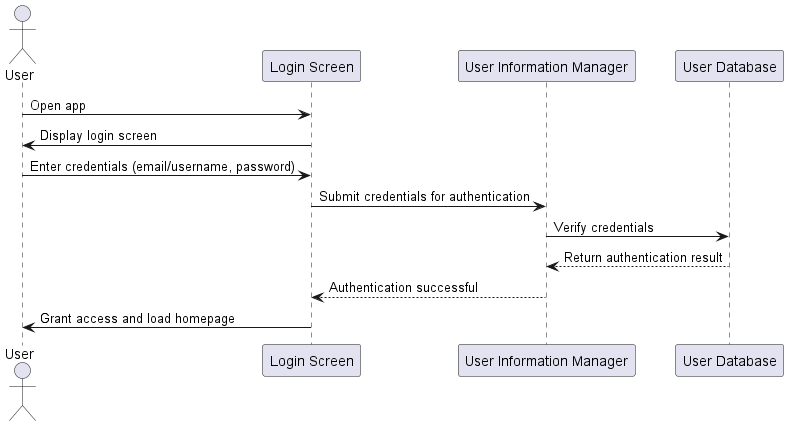
\includegraphics[scale=0.6]{Sequence Diagrams/BE2_Sequence_Diagram.png}\\
	\textbf{Figure 4.} Sequence Diagram for BE2: Authenticate User.\\

	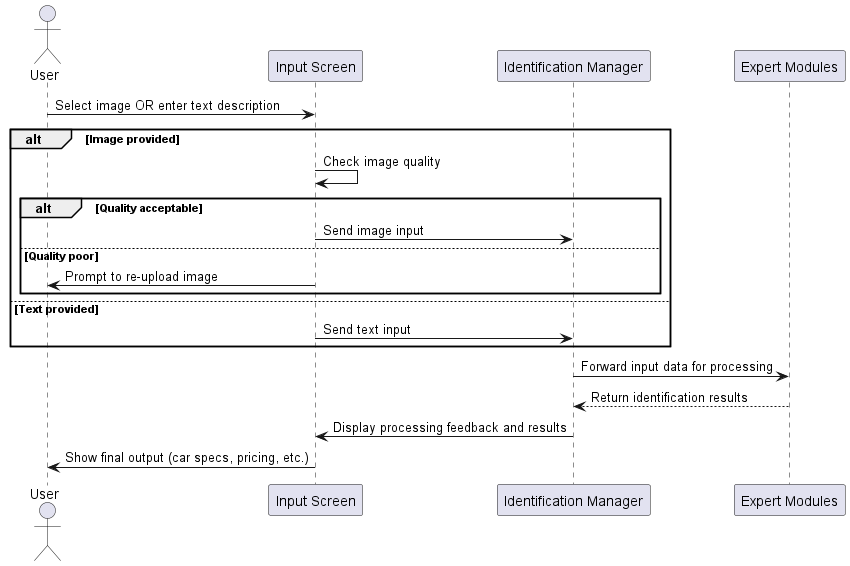
\includegraphics[scale=0.55]{Sequence Diagrams/BE3_Sequence_Diagram.png}\\
	\textbf{Figure 5.} Sequence Diagram for BE3: Upload Text and/or Image as Input.\\

	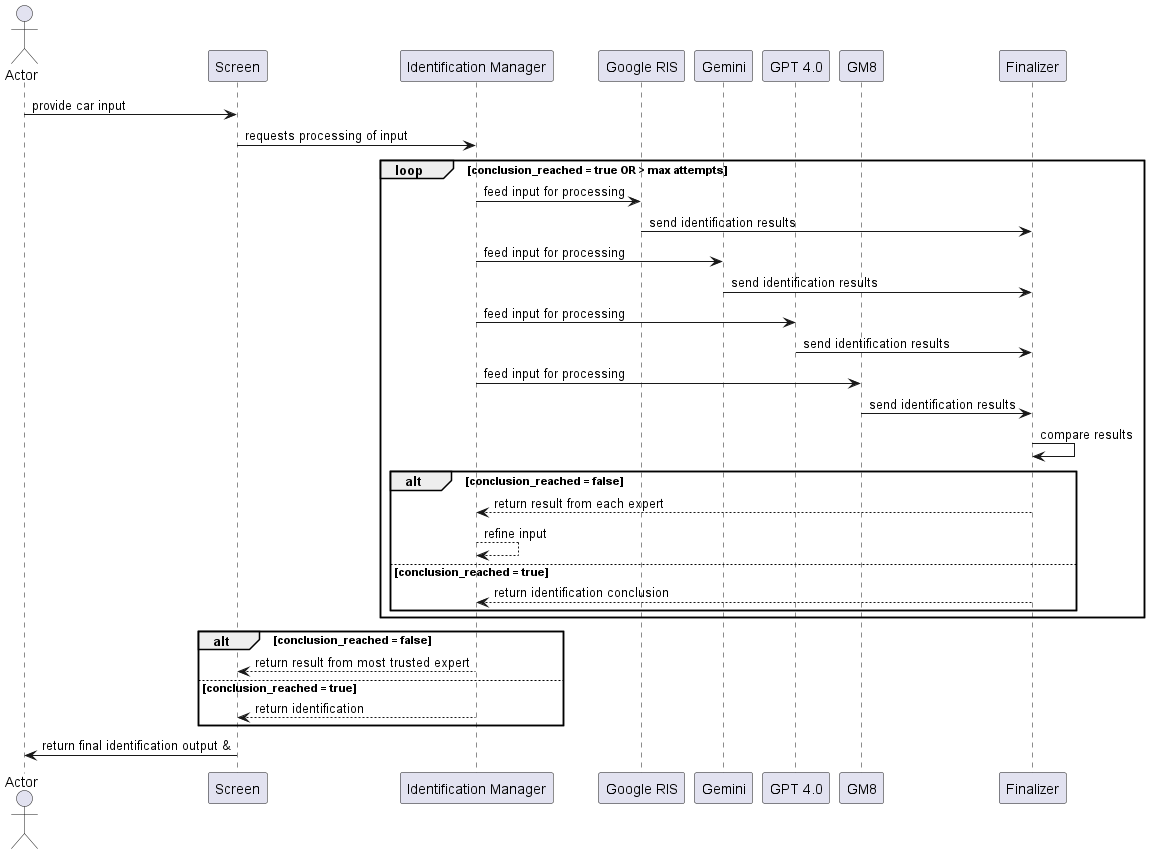
\includegraphics[scale=0.4]{Sequence Diagrams/BE4_Sequence_Diagram.png}\\
	\textbf{Figure 6.} Sequence Diagram for BE4: Compare Expert Answers.\\

	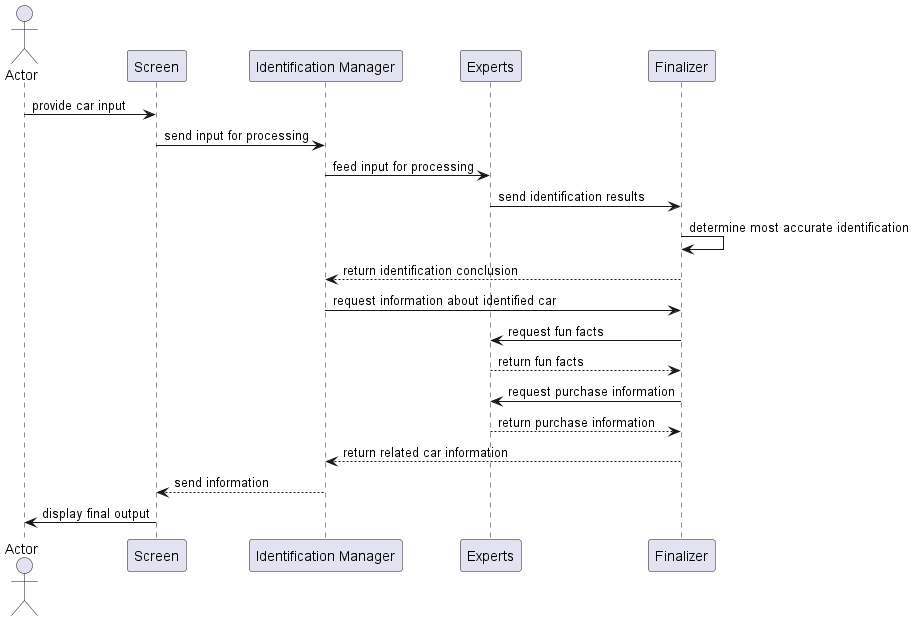
\includegraphics[scale=0.55]{Sequence Diagrams/BE5_Sequence_Diagram.png}\\
	\textbf{Figure 7.} Sequence Diagram for BE5: Present Final Output With Identification Information.\\

	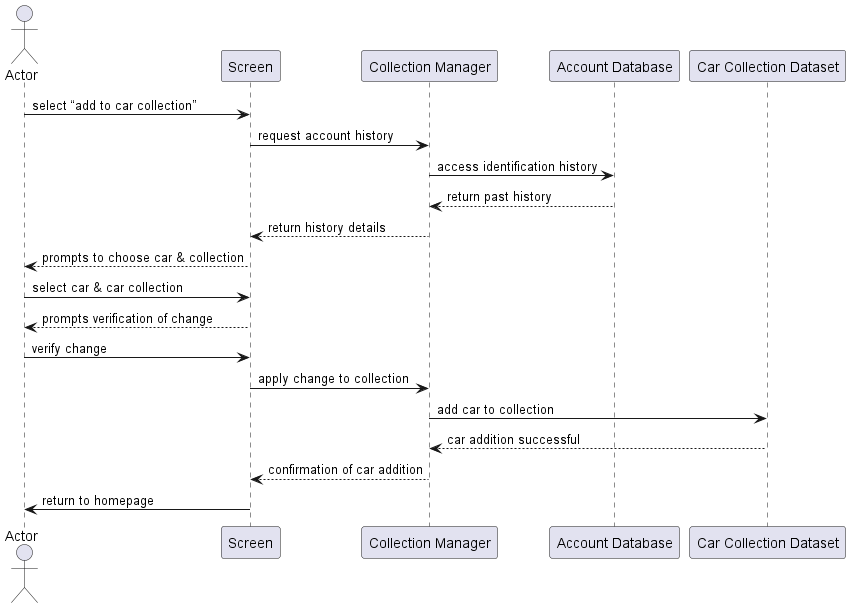
\includegraphics[scale=0.55]{Sequence Diagrams/BE6_Sequence_Diagram.png}\\
	\textbf{Figure 8.} Sequence Diagram for BE6: Add to or Remove From Car Collection.\\
\end{center}
% End Section

\section{Detailed Class Diagram}
\label{sec:detailed_class_diagram}
% Begin Section
\begin{center}
	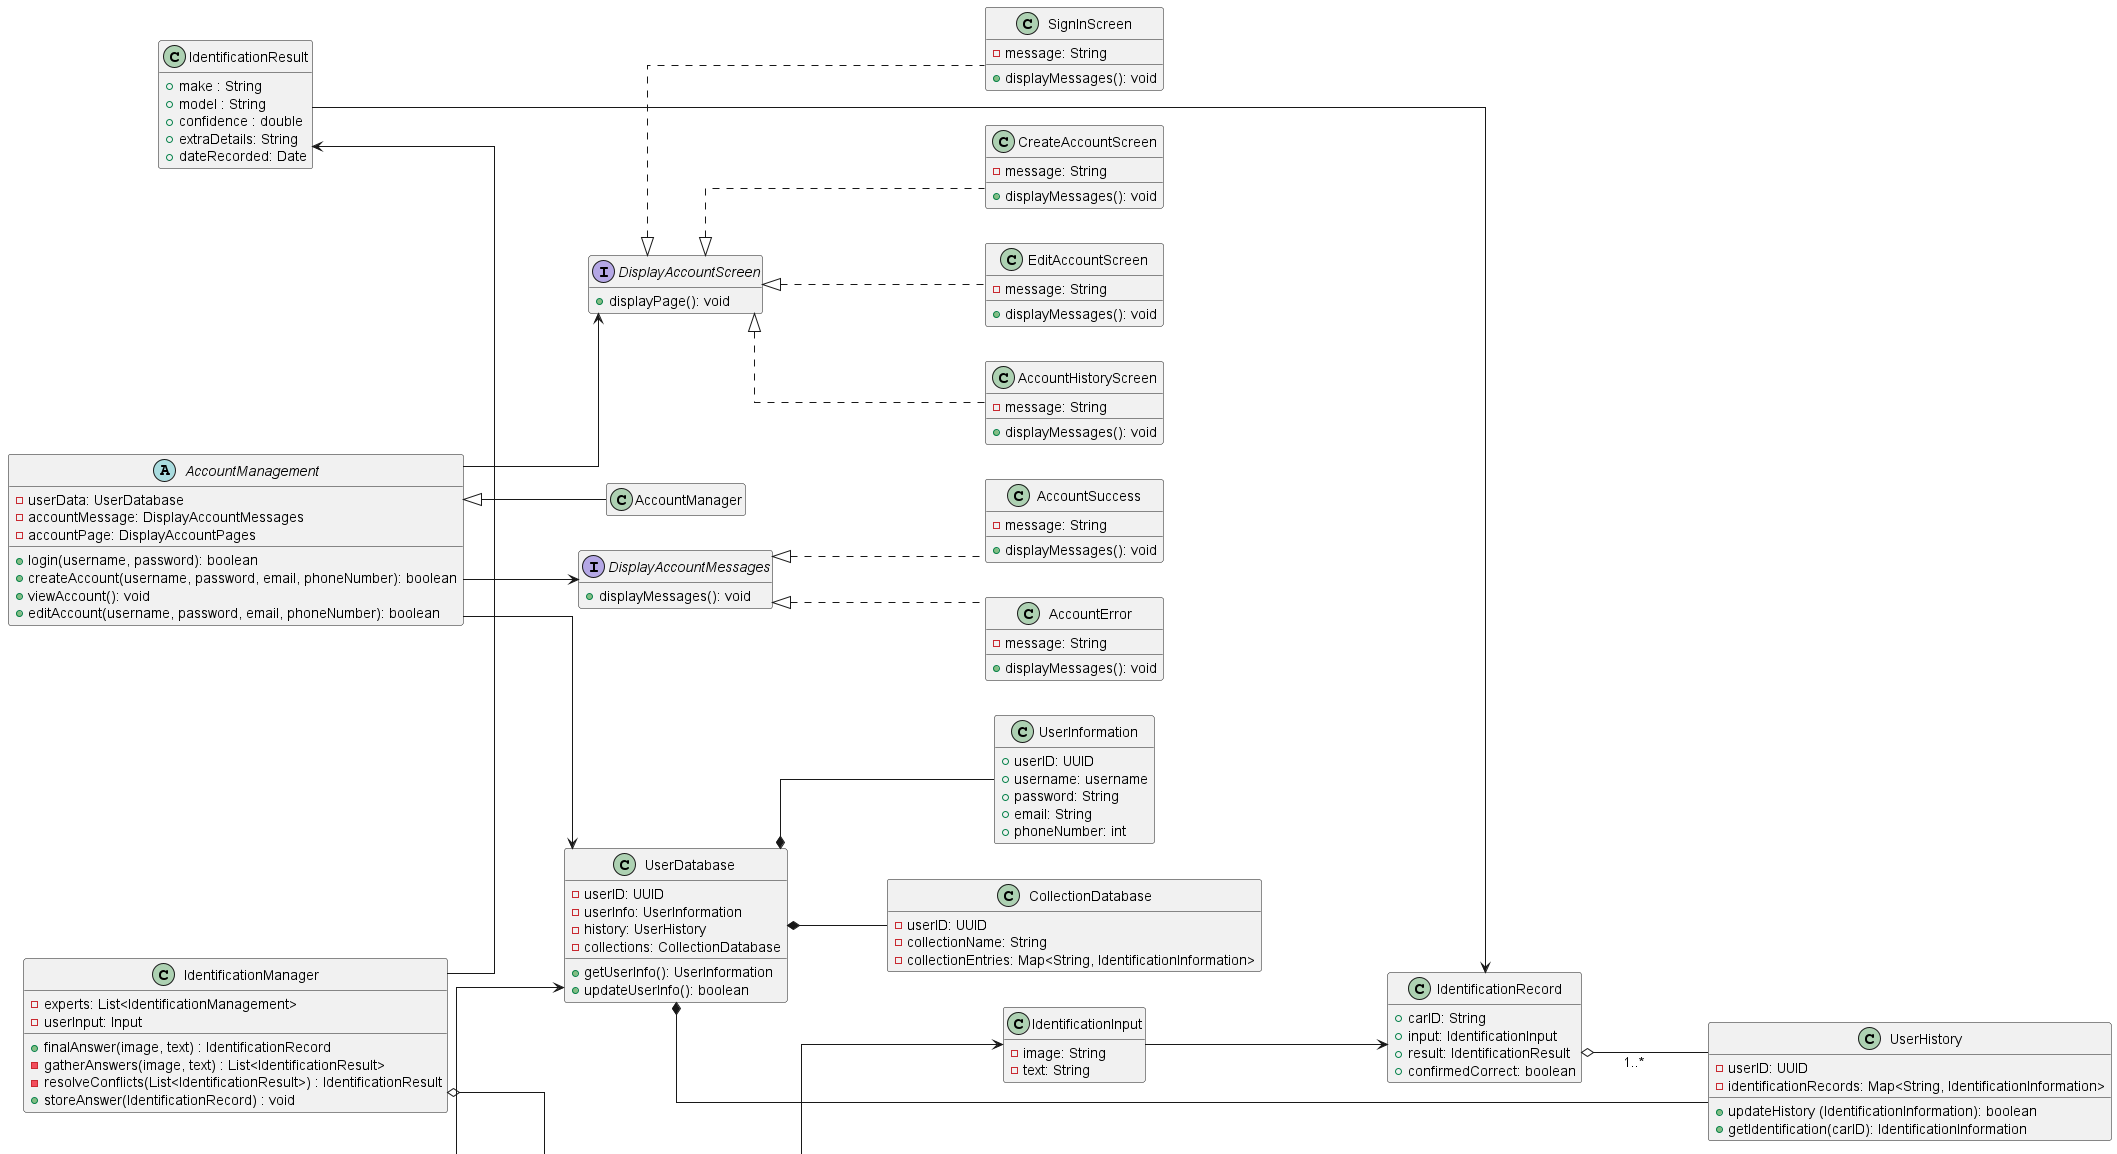
\includegraphics[scale=0.335]{Class Diagram/class_diagram1.png}\\
	\textbf{Figure 9.} First half of detailed Class Diagram of RideRecon system. If blurry, zooming in will clear up the text.\\

	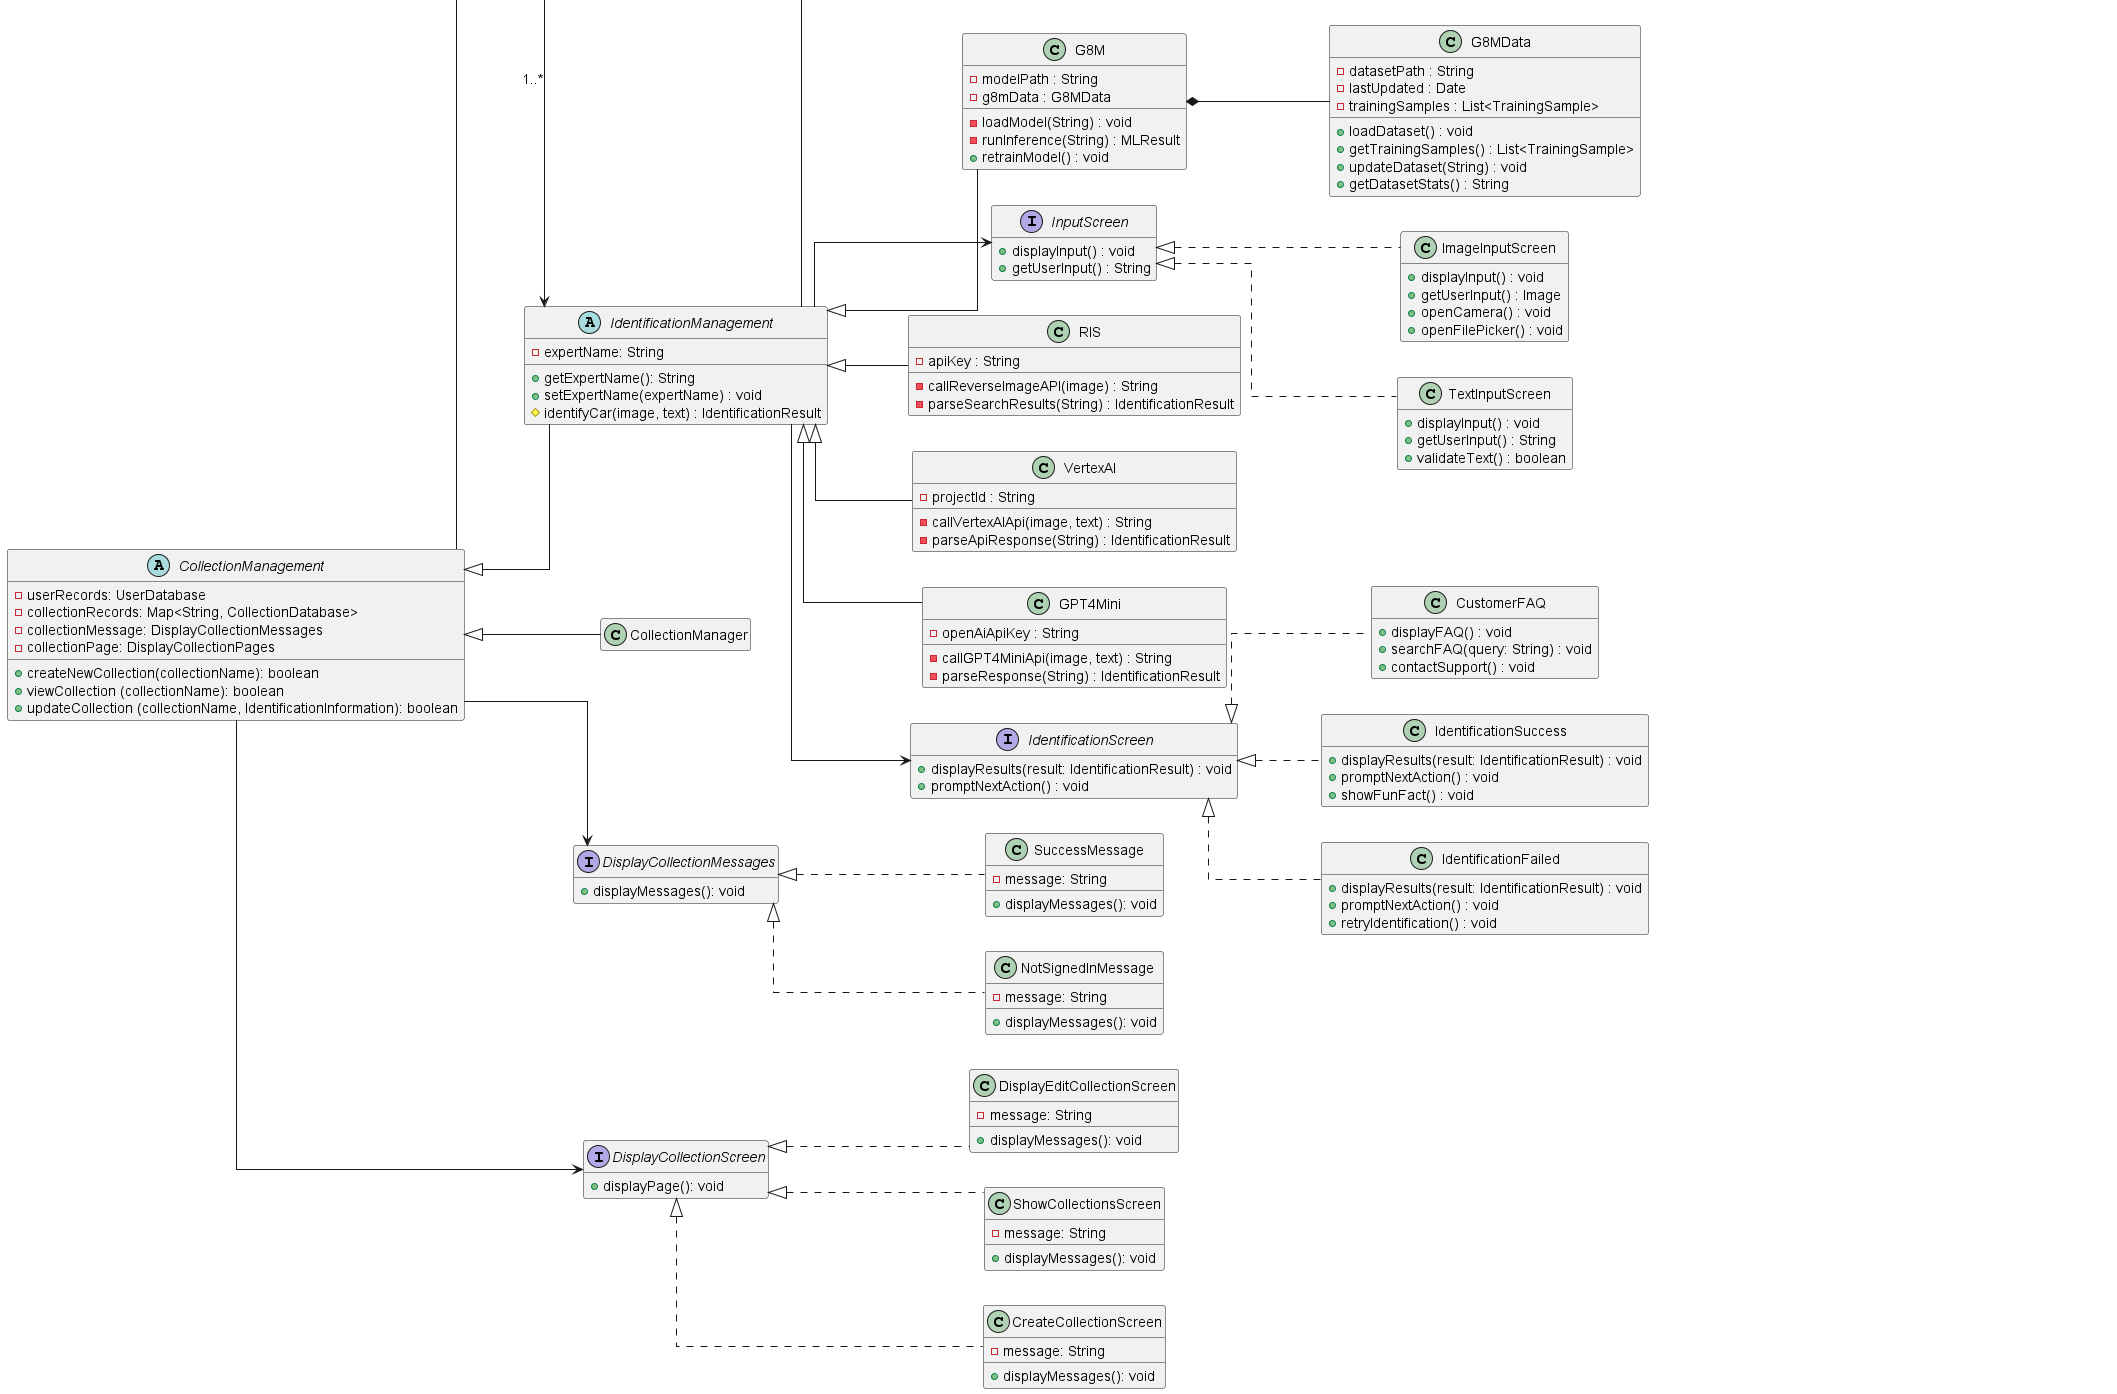
\includegraphics[scale=0.4]{Class Diagram/class_diagram2.png}\\
	\textbf{Figure 10.} Second half of detailed Class Diagram of RideRecon system. If blurry, zooming in will clear up the text.\\

	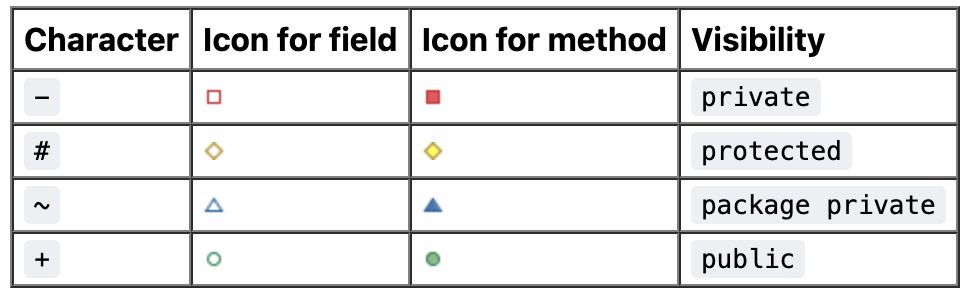
\includegraphics[scale=0.4]{Class Diagram/class_diagram_legend.png}\\
	\textbf{Figure 10.} Legend for detailed Class Diagram of RideRecon system.\\
\end{center}
% End Section

\appendix
\section{Division of Labour}
\label{sec:division_of_labour}
% Begin Section
Include a Division of Labour sheet which indicates the contributions of each team member. This sheet must be signed by all team members.

\begin{table}[h!]
\centering
\begin{tabular}{|p{3.5cm}|p{3.5cm}|p{3cm}|p{3.5cm}|p{3cm}|}
\hline
Hashim Bukhtiar & Jaden Moore & James Ariache & Olivia Reich & Omar Abdelhamid \\ \hline
Section 1.1, 1.2 & Class Diagram in Section 4 & Second State Chart in Section 2 & 3 Sequence Diagrams in Section 3 & Section 1.3 \\ 
3 Sequence Diagrams in Section 3 &  & Helped with Class Diagram in Section 4 & Class Diagram in Section 4 & First State Chart in Section 2 \\
Compiled Final Doc &  &  &  & \\

\includegraphics[height=1cm]{../D1/images/hashim_signature.png} & \includegraphics[height=1cm]{../D1/images/Jaden_signature.jpg} &
\includegraphics[scale=0.1]{../D1/images/james_signature.png}& \includegraphics[height=0.6cm]{../D1/images/olivia_signature.png} & \includegraphics[height=0.6cm]{../D1/images/omar_signature.png}  \\
\hline
\end{tabular}
\caption{Division of Labour} 
\label{tab:division_of_labour}
\end{table}

% End Section

\newpage
\section*{IMPORTANT NOTES}
\begin{itemize}
	\item You do \underline{NOT} need to provide a text explanation of each diagram; the diagram should speak for itself
	\item Please document any non-standard notations that you may have used
	\begin{itemize}
		\item \emph{Rule of Thumb}: if you feel there is any doubt surrounding the meaning of your notations, document them
	\end{itemize}
	\item Some diagrams may be difficult to fit into one page
	\begin{itemize}
		\item It is OK if the text is small but please ensure that it is readable when printed
		\item If you need to break a diagram onto multiple pages, please adopt a system of doing so and throughly explain how it can be reconnected from one page to the next; if you are unsure about this, please ask me
	\end{itemize}
	\item Please submit the latest version of Deliverable 1 and Deliverable 2 with Deliverable 3
	\begin{itemize}
		\item They do not have to be a freshly printed versions; the latest marked versions are OK
	\end{itemize}
	\item If you do \underline{NOT} have a Division of Labour sheet, your deliverable will \underline{NOT} be marked
\end{itemize}


\end{document}
%------------------------------------------------------------------------------